%-*- coding:UTF-8 -*-


\documentclass[UTF8,12pt,twoside,a4paper]{ctexart} %twoside 双面排版,奇偶页的页眉页脚和页边距可以不同

%应用的包——————————————————————————————————————————
\usepackage{fontspec}%字体的包
\newcommand{\tnewroman}{\fontspec{Times New Roman}}
\newcommand{\adobegothicstdb}{\fontspec{Adobe Gothic Std B}}
\newcommand{\Centaur}{\fontspec{Centaur}}
\setmainfont{Times New Roman}%fontspec下这个命令设置全局默认字体


%页眉参考http://www.ctex.org/documents/packages/layout/fancyhdr.htm

\usepackage{graphicx}%插图宏包
\usepackage{caption}%figure legend

\usepackage{setspace}%设置行距的包
%\setlength{\baselineskip}{1.6em}%2倍行距


\usepackage{indentfirst}%首行缩进的包
%\setlength{\parindent}{2em}%首行缩进2

\usepackage{geometry}%设置页边距的包
\geometry{left=2.5cm,right=2.5cm,top=3.5cm,bottom=2.5cm} % 设置页边距


\usepackage{titletoc} %更改目录的包
\titlecontents{section}[3em]%标题位置左间距
{\songti \zihao{-4}\vspace{10pt}}           %设置标题字体是宋体(但是被后面命令覆盖了);字号小四;与上一个标题垂直距离
{\contentslabel{2em}}%设置标题标志的格式,如序号格式、序号宽度、序号与标题内容之间的间距
{\hspace*{-2em}}%设置无序号标题的格式,如字体、字体尺寸、位置等。该参数可以空置
{~\titlerule*[0.6pc]{$.$}~\contentspage}%设置标题与页码之间的指引线样式以及页码的格式,该参数如果空置,标题将无指引线

\titlecontents{subsection}[4em]{\songti\zihao{-4}\vspace{10pt}}{\contentslabel{2em}}{\hspace*{-2em}}{~\titlerule*[0.6pc]{$.$}~\contentspage} %指引线与页码

\usepackage{enumerate} %设置列表环境的包

\usepackage{fancyhdr}  %设置页眉页码的包
\pagestyle{fancy}
\lhead{中山大学高级计算机网络课程论文} %页眉左边
\chead{} %页眉中间
\rhead{边缘计算技术发展综述} %页眉右边
%\lfoot{From: K. Grant} %页脚右边是From: K. Grant
\cfoot{\thepage} %页脚中间是本页页码
%\rfoot{To XXX} %页脚右边是To XXX
\renewcommand{\headrulewidth}{0.4pt} %页眉划线
%\renewcommand{\footrulewidth}{0.4pt}%页脚划线

%\pagestyle{myheadings}
%\markboth{中山大学博士学位论文}{战猇亭先主得仇人~守江口书生拜大将}%设置左边页眉的中山大学博士学位论文,右边页眉是论文标题



\usepackage{afterpage}%更改目录计数的

\usepackage{hyperref}%内部交叉引用



\begin{document}


\setcounter{page}{1}%页码开始计数
\pagenumbering{Roman}%样式有:  arabic, roman, Roman, alph, Alph


%中文摘要——————————————————————————————————————
\begin{titlepage}
    \addcontentsline{toc}{section}{\songti{\zihao{-4}\textbf{摘要}}}
	\begin{center}
		\zihao{-1}\bfseries 边缘计算技术发展综述\\%\zihao{-2}字号-4就是小四;-5就是小五 
		\vspace*{36pt}%行间距增加36pt
		\songti\zihao{-3}
		\begin{tabular}{l}
			{专业:大数据与人工智能}\\
			{学号: 21215122}\\
			{硕士研究生:何峙}\\
			{授课老师:温武少}\\
		\end{tabular}

		\vspace*{36pt}
%\section*{\heiti{\zihao{-2}{摘要}}}
		\heiti{\zihao{-2}{摘要}}
			\vspace*{16pt}
	\end{center}
		
						%\indent\setlength{\parindent}{2em}%首行缩进2字符
	\songti\zihao{-4}
						 %\renewcommand{\baselineskip}{1.6em}
							%\hspace{0.8em}%首段首行缩进
边缘计算作为一种新兴的计算网络架构,它将云计算服务扩展到网络边缘,利用软件和硬件平台,可以应用于移动、无线和有线网络的场景。随着物联网的出现、自动驾驶、VR和AR设备的推出等,使得边缘计算成为关键技术之一。为了理解边缘计算当前存在的挑战与机遇,本文概述了边缘计算技术的基本概念,通过分析边缘计算研究现状和应用场景,指出当前边缘计算在数据存储、数据传送、网络安全等方面的技术要点,并分析它们的优缺点。最后,对边缘计算技术的未来发展进行探讨和展望。

    \begin{flushleft}
        \heiti{\zihao{3}{关键词:}} \songti{\zihao{4}{边缘计算,云计算,边缘智能}}
    \end{flushleft}

\end{titlepage}


%目录————————————————————————————————————————————
\tableofcontents%形成目录
\clearpage{\pagestyle{empty}}
%\clearpage %这一页留空,余下内容直接进入新的一页
%\newpage%插入一个完整的没有内容的空白页
\mbox{}
%\cleardoublepage %这一页留空,余下内容直接进入新的一页


% 正文开始
\setcounter{page}{1}
\pagenumbering{arabic}%阿拉伯数字页码

%—第一章引言———————————————————————————————————————
\addcontentsline{toc}{section}{\textbf{\songti{\zihao{-4}{第一章~引言}}}}
\begin{center}
    \heiti{\zihao{2}{第一章~引言}}
\end{center}
\vspace*{10pt}

% \begin{flushleft}%左对齐开始     flushright则是右对齐
\indent\setlength{\parindent}{2em}%首行缩进2字符
\songti
              %\zihao{-4}
					 %\renewcommand{\baselineskip}{1.5em}
% \hspace{1.6em}%首段首行缩进
智能手机和平板电脑等移动终端的普及对移动网络产生了极大的影响,这给全球移动网络带来了挑战。首先,蜂窝网络要承受低存储容量、高能耗、低带宽和高延迟等缺点。物联网的出现进一步加剧了这种状况。云计算技术通过提供集中的云资源,为终端设备提供相当大的存储和计算能力。然而,随着大量终端设备的出现,云计算正面临着如高延迟、安全漏洞、低覆盖等挑战。另外,云计算不太适用于实时性要求较高的应用和高服务质量的场景。
边缘计算通过将处理带到应用程序的边缘来满足上述云计算适用不了的要求。

目前,云计算问题可以通过若干种边缘计算模型来解决。如欧洲电信标准协会(ETSI)引入的移动边缘计算\cite{RN1},移动用户可以利用来自基站的计算服务。思科引入了雾计算(Fog Computing)\cite{RN2}概念,使应用程序能够通过数十亿个智能连接设备直接在网络边缘上运行。还有Satyanarayanan等引入了Cloudlets\cite{RN3}的概念,通过使用本地网络中可用的计算机资源来解决访问云的延迟问题。所以,边缘计算技术为快速增长的终端设备和数据提供稳定的服务,而且边缘计算离数据源很近,比如智能终端,它在网络边缘存储和处理数据,具有邻近性和位置感知,能较快的为用户提供近端服务。在数据处理方面,它更快、实时且安全。 它还可以解决云计算中的过度能耗问题,降低成本,减轻网络带宽压力。

本文将从以下几个方面阐述边缘计算技术的发展现状:
\begin{itemize}
    \item 第二章主要阐述边缘计算的基本概念,包括其架构与特性,以及与云计算的区别与联系;
    \item 第三章边缘计算的应用场景,了解其中的实现方式;
    \item 第四章总结与展望边缘计算;
\end{itemize}

% \end{flushleft}%左对齐结束
\clearpage


%—第二章~边缘计算基本概念——————————————————————————————

\addcontentsline{toc}{section}{\textbf{\songti{\zihao{-4}{第二章~边缘计算基本概念}}}}
\begin{center}
    \heiti{\zihao{2}{第二章~边缘计算基本概念}}
\end{center}
\vspace*{10pt}
\addcontentsline{toc}{subsection}{\songti{\zihao{-4}{1.概念与技术定义}}}
\begin{flushleft}
    \heiti{\zihao{3}{1.概念与技术定义}}
\end{flushleft}
    % \vspace{5pt}
\indent\setlength{\parindent}{2em}%首行缩进2字符
\songti
\hspace{1.6em}%首段首行缩进
在了解边缘计算概念之前,先回顾一下云计算的概念。云计算是通过网络将所有数据传输到云计算中心,集中解决计算和存储问题。在2006年8月的搜索引擎大会(sessane jose 2006)上,Google首席执行官首次提出了云计算的概念。随着以谷歌为代表的搜索引擎的发展,云计算开始显示出强大的生命力。如今,云计算已经发展得越来越成熟。它是一个非常强大的网络服务平台,包括分布式计算、负载平衡、并行计算、网络存储、虚拟化等技术。然而,随着物联网在人们生活中的出现与发展,接入物联网的设备数量逐渐增加,产生了大量的数据。云计算的网络带宽逐渐无法满足数据处理实时性能的需求。因此,云计算模型在负载、实时性、传输带宽、能耗以及数据安全和隐私保护等方面存在很大缺陷。

不同于传统的云计算,边缘计算是一种在网络边缘执行计算的新计算范式。其核心思想是使计算更接近数据源。Satyanarayanan等\cite{RN3}将边缘计算描述为:“边缘计算是一种新的计算模型,它将计算和存储资源部署在网络边缘,以靠近移动设备或传感器”。而Zhao Ziming等\cite{RN4}则认为:“边缘计算是一种新的计算模型,它将地理距离或网络距离接近用户的资源统一起来,为应用服务提供计算、存储和网络。”Shi Weisong等\cite{RN5}也介绍了边缘计算中边缘的概念:“边缘是指数据源与云计算中心路径之间的任意计算和网络资源。”根据中国边缘计算产业联盟的定义\cite{RN6},边缘计算是“在网络边缘或数据源附近,一个集成网络、计算、存储、应用等核心功能的开放平台,并在附近提供边缘智能服务,以满足连接、实时业务、数据优化等行业敏捷性关键要求,以及应用程序智能、安全和隐私”。综上,边缘计算就是在网络和网络的边缘提供服务和执行计算。

边缘计算与云计算互相区别又互相联系。在网络、商务、应用、智能等方面,二者共存、互补、协调发展。边缘计算是云计算的延伸,它与云计算各有其的特点。云计算的主要特点是能够把握全局,能够处理大量数据进行深入分析,并且在业务决策等非实时数据处理领域发挥着重要作用。而边缘计算专注于本地,可以在小规模、实时智能分析中发挥更好的作用,如满足本地企业的实时需求。譬如,在智能应用中,云计算更适合大规模数据的集中处理,而边缘计算可以用于小规模智能分析和本地服务。在网络资源方面,边缘计算负责更接近信息源的数据。因此,数据可以在本地存储和处理,而无需将所有数据上传到云端。网络负担的减轻大大,提高了网络带宽的利用效率。

云计算和边缘计算在未来智能物联网的发展中发挥着重要作用。边缘节点上的所有数据仍然需要在云中进行汇总,以实现深入分析并获得更有意义的分析结果。因此,云计算仍然在逐渐智能化的物联网设备的发展中发挥着重要作用。在物联网的背景下,如果连接设备产生的所有大量数据都传输到云,云计算将造成巨大的负载。此时,边缘计算需要分担云的压力,并负责边缘范围内的任务。当边缘计算出现问题时,数据不会在云平台中丢失。在一些互联网服务中,数据经过边缘计算处理后需要返回到云进行处理,比如数据挖掘和共享的数据分析,这需要云计算和边缘计算的互相协作。两者发展都为物联网中的连接设备带来了稳定性。两者的工作方式可以是云计算基于大数据分析和输出,将数据传递到边缘端,然后由边缘计算处理和执行。如今,两者的协调发展已经应用于现实生活的许多方面,如智能制造、能源、安全和隐私保护以及智能家庭 。例如,在智能制造的工业生产中,云计算的作用是控制整体。在边缘节点中,需要具有实时检测和及时解决问题的功能。边缘计算利用了实时性的特点,与云计算合作,不仅提高了生产效率,还可以及时检测设备的异常情况。在智能家居领域,边缘计算节点主要涉及一些智能终端。边缘计算节点计算来自不同设备的异构数据并上传到云端进行处理,从而实现对云端边缘节点的控制和边缘节点对云端的访问。为了满足物联网设备的需求,云计算和边缘计算发挥各自的优势,只有两者的共同发展才能不断推动互联网的进步。
\vspace{10pt}

\addcontentsline{toc}{subsection}{\songti{\zihao{-4}{2.边缘计算基本架}}}
\begin{flushleft}
    \heiti{\zihao{3}{2.边缘计算基本架构}}
\end{flushleft}
\indent\setlength{\parindent}{2em}%首行缩进2字符
\songti
\hspace{1.6em}%首段首行缩进
边缘计算架构是一种联邦网络结构,通过在终端设备和云计算之间引入边缘设备,将云服务扩展到网络边缘。云边缘协作的结构由下到上一般可以分为以下三层:
\begin{itemize}
    \item 终端层

    终端层由连接到边缘网络的所有类型的设备组成,包括移动终端和许多物联网设备(如传感器、智能手机、智 能汽车、摄像头等)。在终端层,设备不仅是数据消费者,也是数据提供者。为了减少终端服务延迟,只考虑各种终端设备的感知,而不考虑计算能力。因此,终端层的数亿台设备收集各种原始数据并上传到上层,在那里存储和计算数据。
    
    \item 边界层

    边界层是三层体系结构的核心。它位于网络的边缘,由广泛分布在终端设备和云之间的边缘节点组成。它通常包括基站、接入点、路由器、交换机、网关等。边界层 支持终端设备向下访问,并存储和计算终端设备上传的数据。连接云端,将处理后的数据上传到云端。由于边界层距离用户较近,因此到边界层的数据传输更适合实时数据分析和智能处理,比云计算更高效、更安全。
    
    \item 云计算层
    
    在云边缘计算的联邦服务中,云计算仍然是最强大的数据处理中心。云计算层由多台高性能服务器和存储设备组成,具有强大的计算和存储能力,可以在需要大量数据分析的领域发挥良好作用,如定期维护和业务决策支持。云计算中心可以永久存储边缘计算层的报告数据,还可以完成边缘计算层无法处理的分析任务和集成全局信息的处理任务。此外,云计算模块还可以根据控制策略动态调整边缘计算层的部署策略和算法。
\end{itemize}

如图1的Ju Ren等\cite{RN7}在可扩展的物联网架构中总结的边缘计算网络架构就比较好的概括了边缘计算网络层次。
\begin{figure}[htbp]%htbp作为浮动体,可以出现在周围文本所在处和一页的顶部
	\centering%内容居中\raggedleft左对齐
	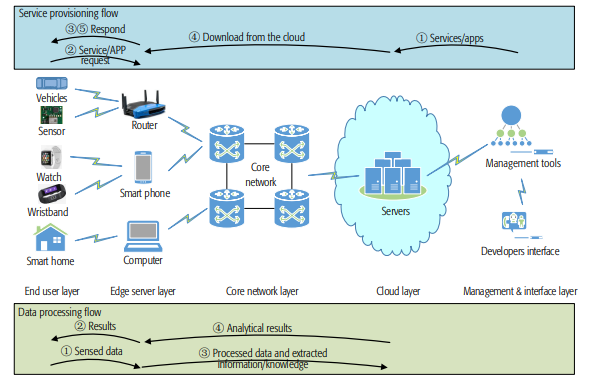
\includegraphics[scale = 1.0]{pic1.png}%scaale就是缩放倍数
	\caption*{\zihao{5} \songti 图1 边缘计算基本架构\cite{RN7}}
\end{figure}
\vspace{10pt}

\addcontentsline{toc}{subsection}{\songti{\zihao{-4}{3.边缘计算特性}}}
\begin{flushleft}
    \heiti{\zihao{3}{3.边缘计算特性}}
\end{flushleft}%左对齐结束

\songti

\begin{itemize}
\item 密集的地理分布

边缘计算通过在边缘网络中部署大量计算平台,使云服务更接近用户基础设施的密集地理分布有助于网络管理员可以促进基于位置的移动服务,而无需穿越整个广域网,另外也使大数据分析可以更快、更准确地执行。而且,边缘系统能够实现大规模的实时分析。

\item 可移动性

随着移动设备数量的快速增长,边缘计算也支持移动,如定位器ID分离协议(LISP ),以直接与移动设备通信。LISP协议将位置标识与主机标识分离,并实现了一个分布式目录系统。主机身份与位置身份的分离构成了边缘计算中支持移动性的关键原则。 

\item 位置感知

边缘计算的位置感知属性允许移动用户从距离其物理位置最近的边缘服务器访问服 务。用户可以使用各种技术,如手机基础设施、GPS或无线接入点来查找电子设备的位置。这种位置感知可用于多个边缘计算应用,例如基于边缘设备的车辆安全应用和基于边缘的 灾难管理。 

\item 本地化

在边缘计算中,计算资源和服务在用户附近可用,可以改善他们的体验。本地附近计算 资源和服务的可用性允许用户利用网络上下文信息做出卸载决策和服务使用决策。类似地, 服务提供商可以通过提取设备信息和分析用户的行为来利用移动用户的信息,以改进他们的 服务和资源分配。

\item 低延迟

边缘计算范式使计算资源和服务更接近用户,从而减少了访问服务的延迟。边缘计算的低延迟使用户能够在资源丰富的边缘设备上执行资源密集型和延迟敏感型应用程序。

\item 上下文感知

移动设备可以根据位置感知进行定义。边缘计算中移动设备的上下文信息可用于做出卸载决策和访问边缘服务。实时网络信息,如网络负载和用户位置,可以用来为边缘用户提供上下文感知服务。此外,服务提供商可以使用上下文信息来改善用户满意度和体验质量。 

\item 异质性

边缘计算中的异质性指边缘计算元素(终端设备、边缘服务器和网络)使用的各种平台、架构、基础设施、计算和通信技术。在终端设备的异质性中,软件、硬件和技术的变化构成了异质性的主要因素。边缘服务器端的异构性主要是由API、定制策略和平台造成的。这种存在的差异导致互操作性问题,并使其成为边缘计算成功部署的主要挑战。
\end{itemize}

%\cleardoublepage %这一页留空,余下内容直接进入新的一页
\clearpage{\pagestyle{empty}}%空余一页,余下内容直接进入下一页,而且不要出现页眉页码

%—第三章~边缘计算应用场景——————————————————————————————
\addcontentsline{toc}{section}{\textbf{\songti{\zihao{-4}{第三章~边缘计算应用场景}}}}
\begin{center}
    \heiti{\zihao{2}{第三章~边缘计算应用场景}}
\end{center}
\vspace*{10pt}
\addcontentsline{toc}{subsection}{\songti{\zihao{-4}{1.工业物联网}}}
\begin{flushleft}
    \heiti{\zihao{3}{1.工业物联网}}
\end{flushleft}
    % \vspace{5pt}
\indent\setlength{\parindent}{2em}%首行缩进2字符
\songti
\hspace{1.6em}%首段首行缩进
工业物联网是一种将机器、计算机和人员使用业务转型所取得的先进的数据分析成果相结合,从而达到智能化的工业运营。在工业物联网的实际应用中,不仅需要高度的精确度和安全性,而且需要对整个行业的运行过程进行实时的监测和控制。因此,在工业物联网中实现移动边缘计算成为必然的选择。具体来说,主要有以下几个优势:第一、提高性能。在 MEC服务器上实现了对工业生产过程中的报警、故障分析等方面的分析,从而提高了数据的处理速度、做出了正确的判断、提高了系统的运行效率和提高了边缘处理的灵活性;第二、保证数据的安全与隐私。在 MEC服务器上进行数据处理,大概率避免了远程传输时的数据泄露。第三、减少操作成本。在边缘进行运算,降低了数据中心和边缘设备的数据传输和传输带宽,降低了网络、云端数据中心的计算和存储费用。因此,边缘计算在工业物联网中的应用是非常有意义的。
\vspace{10pt}

\addcontentsline{toc}{subsection}{\songti{\zihao{-4}{2.车联网}}}
\begin{flushleft}
    \heiti{\zihao{3}{2.车联网}}
\end{flushleft}
\indent\setlength{\parindent}{2em}%首行缩进2字符
\songti
\hspace{1.6em}%首段首行缩进
提到车联网,就不得不提无人驾驶,作为一项技术革新的新技术,无人驾驶集合了现代传感技术、信息通信技术、自动控制技术、计算机技术和人工智能技术,是当今汽车技术发展的一个重要趋势,也是当前汽车工业发展的一个重要趋势。所以,无人驾驶系统是非常精密的,它包含很多技术,包括感知,定位,感知,决策,以及与云端平台进行流畅的互动,以便产生高清晰度的地图和数据储存。即便有如此多的专业感应器及其他专业仪器,但在某些特殊状况下,仍无法有效地解决某些交通事故中的安全隐患。比如,如果是在超视距范围内,如果汽车上有雷达、摄像机等传感器无法探测到拐弯处的车辆,或是有一辆汽车从拐角处开来,那么很可能会引发车祸。

从交通效率的角度来说,对于交通部门,提高交通效率是他们的首要任务。但是,当无人驾驶汽车在路上行驶时,出于安全考虑,会采取相对保守的措施。比如说,它的行驶速度会很慢,遇到意外的话,会减速,或者是停车,这就导致了交通的效率下降。	

由此可见,无人驾驶智能决策的时延要求非常高,如果将大量的基于计算机视觉或者雷达数据的路况实时分析移到云端去计算,这样会导致更多的时间延迟,从而对车辆的性能产生很大的负面作用。这就给了边缘计算很大的发展契机,把云端那些计算任务移到路侧的边缘计算平台上来进行,通过在路侧的基础设施上部署边缘计算平台和车联网的应用,从而对车辆进行实时的智能提醒和决策。这种算法在接近于互联网访问的道路上进行边界运算,其优势显而易见:第一,运算速度大大提高,有助于提高精确性;第二,不会消耗太大的核心网和核心网的带宽;第三,可以减少延迟,在网络的边沿,只需要在基站的帮助下,就可以向道路上的各个节点发送信息。

具体来说,汽车终端经由5G基站与5G核心网连接,最后到达在因特网上部署的各类服务。在此基础上,将核心网络划分为:控制面板装置CCF和用户界面装置UPF。在5G网络中,有许多功能实体,它们是专门用于5G网络的核心网元。MEC必须在边缘 UPF附近部署,并利用本地转移功能,把客户的业务需求转移到MEC,然后由MEC中的应用程序来完成。在MEC中,业务被配置在靠近边缘UPF的位置,其数据的传送路径显著缩短。当使用者访问一个边缘应用时,使用者的请求会透过局部分流,直接传送至位于基地站一侧的MEC,使其数据可以在网路边缘进行处理,而不会影响后端核心网路的网路带宽,并可减少移动网路的延迟,其优点是非常明显的。

对于车路协同系统,通过设置摄像机和毫米波雷达进行实时监测,并根据实时的行人位置和交通信号的状况,向司机发送红色或者接近车道的行人信息,帮助司机作出相应的减速判断。同时,边缘云还能向中央云报告初步分析的行人数据,由中心云通过大数据对行人的行为进行预测,并将距离较远但正在接近的行人信息发送给车辆司机,从而进一步减少事故的发生。
\vspace{10pt}

\addcontentsline{toc}{subsection}{\songti{\zihao{-4}{3.智能家居}}}
\begin{flushleft}
    \heiti{\zihao{3}{3.智能家居}}
\end{flushleft}%左对齐结束
\indent\setlength{\parindent}{2em}%首行缩进2字符
\songti
\hspace{1.6em}%首段首行缩进
在智能家居场景中,通过自然语音和终端设备进行交互已经成为当前行业的主流。由于家庭场景的特殊性,家庭终端需要精确地识别和提取正确的用户指令、声源、声纹等信息,因此智能家居领域的语音交互对边缘计算的要求也越来越高。譬如,家庭中的声音很复杂,有电视的声音、多人的对话、孩子们的嬉戏、空间的回响(厨房做饭、洗衣机等设备的工作噪声),都有可能同时出现,所以必须要处理和抑制各种干扰,让真实使用者的声音变得更加清晰。在此过程中,设备所需的信息将会更多地用于辅助决策。在家庭环境中,语音交互的一项基本功能就是利用话筒阵列进行多信道的同步输入,并对其进行分析,从而提高语音的空间位置,从而提高语音的质量。另外,它还可以利用声纹信息帮助识别真实使用者,让使用者在多人干扰的情况下,更容易分辨。这些都是在设备上进行的,而且对计算能力的要求也很高。另外,特定场景中用户常用的关键字指令数量是有限的,例如音乐产品,用户使用频率最高的可能是“上一次/下一次”,空调产品中最常用的命令是“开/关”等等。对于高频词的处理,完全可以将其放到本地处理而不依赖于云端延迟,从而为用户带来最佳体验。这些场景对于边缘计算来说,也是非常适用的。Yar等\cite{RN8}在资源有限的 Raspberry Pi (RPI)设备上,实现了智能住宅自动化系统。RPI作为一个集中控制装置,为家庭内的各类装置和各种传感器的连接提供了一个经济有效的平台,并提出了一种基于物联网与边缘计算的范式。
此外,随着物联网系统中传感器的数量的增加,尽管更多设备的交互给家庭智能化带来好处,但这些物联网设备防止滥用的安全性较弱,经常被滥用来创建分布式拒绝服务(DDoS)攻击。Huraj等\cite{RN9}探讨了如何利用边缘计算的传感器抵抗DDOS攻击。作者通过对IoT传感器的直接管理和对IoT传感器进行控制的智能家庭的个人助理系统的入侵进行了实例分析,对一个单一的攻击进行了试验,展示了一个真实的物联网传感器对 DDoS攻击的抗性并提出解决方案。
\vspace{10pt}

\addcontentsline{toc}{subsection}{\songti{\zihao{-4}{4.增强现实和虚拟现实(AR/VR)}}}
\begin{flushleft}
    \heiti{\zihao{3}{4.增强现实和虚拟现实(AR/VR)}}
\end{flushleft}%左对齐结束
\indent\setlength{\parindent}{2em}%首行缩进2字符
\songti
\hspace{1.6em}%首段首行缩进
AR/VR技术的出现彻底改变了用户与虚拟世界的交互方式,为了保证用户体验,VR中的图像渲染需要实时性强。研究表明:将VR中的计算任务卸载到边缘服务器或者移动设备上,可以降低处理时延。Li等\cite{RN10}提出了一个这边缘服务器上处理多VR应用的框架——MUVR,作者利用渲染的VR帧之间的冗余,通过自适应地重用为不同VR用户渲染的冗余VR帧,每帧中的这种冗余是由边缘云在运行时决定的,然后边缘云能够记住以前的VR帧渲染结果,以供其他用户将来重用。生成VR帧后,边缘云将与其他帧相比,进一步重用其冗余像素,并且仅将该帧的不同部分传输到移动设备。Lai等\cite{RN11}提出的Furion是一个移动VR框架,它采用在手机和边缘服务器上运行的拆分渲染器架构,将VR负载分为前景交互和背景环境两大类,前景交互仍然在云端进行,背景渲染则由移动端卸载,从而实现移动设备上的VR高质量应用。
\vspace{10pt}

以上只是当前众多边缘计算应用场景中比较热门的大型应用实例,深入到每个主题下,还有许多用例可以探索。 
\vspace{10pt}

%\cleardoublepage %这一页留空,余下内容直接进入新的一页
\clearpage{\pagestyle{empty}}%空余一页,余下内容直接进入下一页,而且不要出现页眉页码


%—第四章~总结与展望——————————————————————————————
\addcontentsline{toc}{section}{\textbf{\songti{\zihao{-4}{第四章~总结与展望}}}}
\begin{center}
	\heiti{\zihao{2}{第四章~总结与展望}}
\end{center}
\vspace*{10pt}
\songti
\hspace{1.6em}
为了追求高性能、低延迟的用户体验,越来越多的计算重任逐渐的由云端推向本地端,随之也出现了双端协同运作的问题,而边缘计算已经被广泛的认为解决这一系列问题的较好的方案。随着大数据的推进和人工智能技术的发展,边缘计算也可以与人工智能相结合,譬如出现了一些智能边缘或成为边缘AI,还有AIoT(Artificial Intelligence of Things)等技术,是十分值得去深究的。

%\cleardoublepage %这一页留空,余下内容直接进入新的一页
\clearpage{\pagestyle{empty}}%空余一页,余下内容直接进入下一页,而且不要出现页眉页码

%—参考文献——————————————————————————————
\addcontentsline{toc}{section}{\textbf{\songti{\zihao{-4}{参考文献}}}}
\renewcommand{\refname}{\zihao{2}{参考文献}}
\bibliographystyle{IEEEtran} %声明参考文献格式为plain,也可以选unsrt,alpha,abbrv等
\bibliography{ComputerNetwork.bib}%参考文献从命名为NHH的bib文件中出


%\cleardoublepage %这一页留空,余下内容直接进入新的一页
\clearpage{\pagestyle{empty}}%空余一页,余下内容直接进入下一页,而且不要出现页眉页码




\end{document}




















